\section{Acoustic properties of beatbox sounds}
The most basic and fundamental beatboxing sounds includes the ones imitating kick (also known as bass drum), snare and hi-hat of a drum-machine {Stowell2010}. These sounds can be inspected through waveforms and spectrograms, in return for a better understanding of how the sounds relate and differ from each other. Below is a representation and description of the three mentioned sounds. \\

\begin{figure}[h]
	\begin{center}
		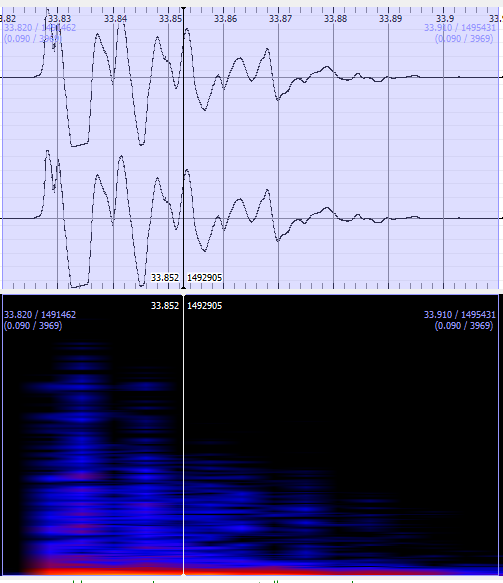
\includegraphics[scale = 0.5]{fig/Kick-closeup-with-spectrogram.png}
		\caption{Kick sound in waveform and in spectrogram(low frequency in the bottom of the spectrogram and high frequency in the top), made with Sonic Visualizer}
		\label{KickClose}
	\end{center}
\end{figure} 

\begin{flushleft}
What can be seen on figure \ref{KickClose} is the kick sound. One can see that the kick sound has low frequencies, because the waveform does not cross the zero line that often, and in the spectrogram one can see more color in the bottom which is the low frequency.\\ 
\end{flushleft}

\begin{figure}[H]
	\begin{center}
		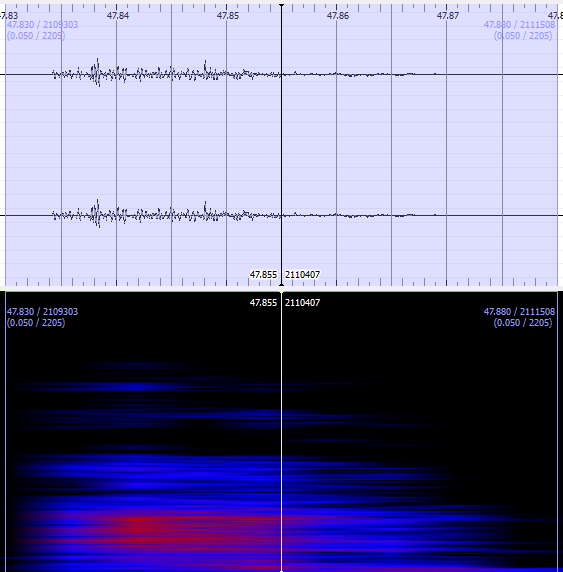
\includegraphics[scale = 0.5]{fig/Snare-close-up-with-spectrogram.png}
		\caption{Snare sound in waveform and in spectrogram(low frequency in the bottom of the spectrogram and high frequency in the top), made with Sonic Visualizer}
		\label{snareClose}
	\end{center}
\end{figure}

\begin{flushleft}
Figure \ref{snareClose} presents a close up of the waveform of the snare sound. It can be seen that the sound has higher frequencies, and the spectrogram shows more colors closer to the top. 
\end{flushleft}
\begin{figure}[H]
	\begin{center}
		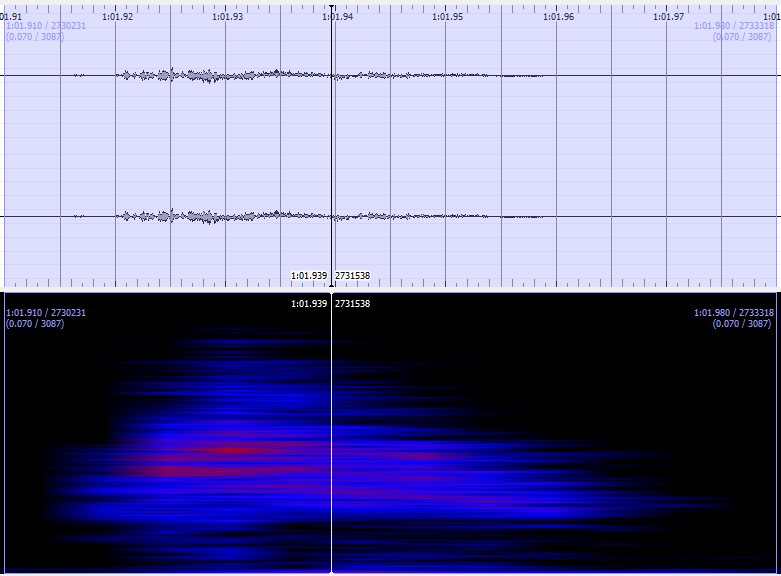
\includegraphics[scale =  0.5]{fig/HH-close-up-with-spectrogram.png}
		\caption{Hi-hat sound in waveform and in spectrogram(low frequency in the bottom of the spectrogram and high frequency in the top), made with Sonic Visualizer}
		\label{HHClose}
	\end{center}
\end{figure}
Lastly is the hi-hat sound, and as seen on figure \ref{HHClose} hi-hat also has higher frequencies than the kick drum beatboxing sound. It also contains slightly higher frequencies than the snare drum. For an easier compression of the 3 sounds one can look at figure \ref{HH-Snare-Kick}.
\begin{figure}[H]
	\begin{center}
		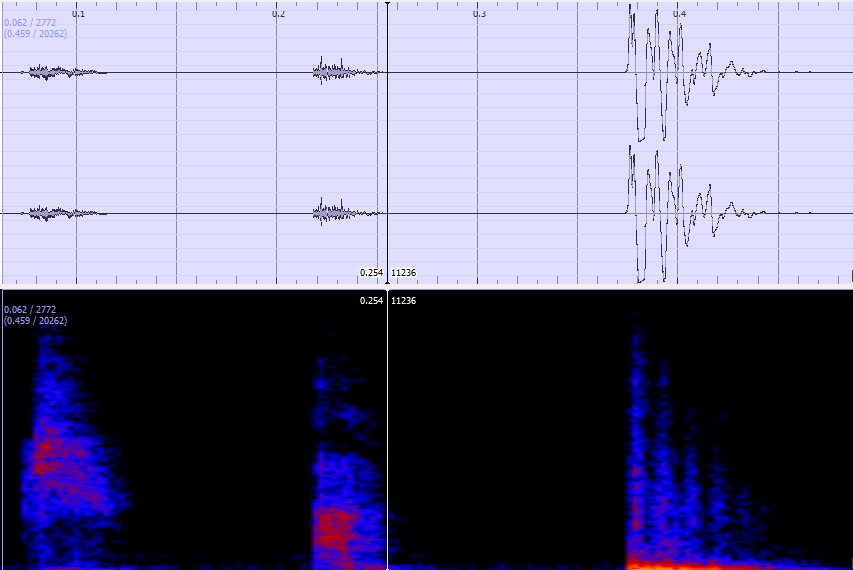
\includegraphics[scale =  0.5]{fig/hh-snare-kick-with-spectogram.png}
		\caption{Hi-Hat, snare and kick sound in waveform and in spectrogram(low frequency in the bottom of the spectrogram and high frequency in the top), made with sonic visualizer}
		\label{HH-Snare-Kick}
	\end{center}
\end{figure}
What we can conclude from this is that the three sounds look different with the greatest difference in the kick compared to snare and hi-hat.